\section{2026년 3월 3일, 20시 18분, 흐림}
안녕 프레키야. 집사가 집을 떠난지 벌써 하루가 지났구나. 세상 어떤 고양이들보다 귀여운 고양이인 너를 두고 집사가 집을 나서 
기숙사로 향하는 차를 탈 때부터 네 생각을 계속 했단다.
슬픈 일이지만 집사가 너를 이제 자주 보지 못할 수도 있게 되었어. 아빠가 집사와 사실상 절연을 선언하고 집사는 이제 네가 있는 집으로 돌아가기가 힘들게 되었단다. 
그래서 집사가 네가 보지도 읽지도, 설사 보더라도 이해하지 못할 사람의 말로 매일 편지를 쓰려고 해. 언제 다시 너를 볼 수 있게 될지는 모르겠지만 
조속히 집이든 아니든 어디서든간에 너를 보고 꼭 안아주고 싶구나. (네가 안기는걸 정말 끔찍히 싫어하는건 알지만 그래도)

사실 집사는 이 상황이 정말 막막하단다. 사실 집사는 태어나고 23년을 살았는데 인간이 혼자 상서기에 24살은 너무 어린 나이라고 생각하거든. 
고양이인 네가 이해하긴 힘들겠지만 인간은 그렇단다.
그래서 지금 당장은 집사가 뭘 해야 할지 모르겠어. 아빠한테 용서를 빌어야 할지, 아니면 아빠 말대로 일찍 홀로 서서 꾸역꾸역 힘겹게 살아가야 하는지. 
돈이 절실히 필요한 상황에서 지금 다니고 있는 대학을 때려치고 당장 일자리를 구해야 할지, 아니면 졸업은 하고 더 좋은 일자리를 찾아야 할지.
그냥 모든게 막막하구나. 너는 이해하기 힘들겠지만 인간들 사이에선 이런 일도 일어난단다. 정말 이해하기 힘들지?

하지만 모든걸 포기하진 않을거야. 집사는 어떻게든 프레키 너를 보기 위해 어떻게든 노력할거고, 그게 언제가 되었든 반드시 프레키 네가 건강하게 자라고 있는지 
보기 위해 어떻게든 살아갈거란다. 지금은 갑작스럽게 닥친 이 상황에 눈물이 멈추지 않고 있지만, 집사는 프레키 너를 생각하면서 내일부터는 어떻게든 버텨보려 해.

집사가 항상 말하듯이, 네가 40살이고 50살이고 오래오래 아프지 말고 건강하게 장수한 고양이가 되었으면 좋겠구나. 집사가 언젠가는 너를 볼 수 있게 노력할게. 그 전까지
아프지 말고, 집사를 잊어버리지 말고, 집사처럼 아빠 속 썩이지 말고, 사료 그릇에 밥이 없으면 예은 언니한테 보채야 한다. 알겠지? 
언제까지 이걸 쓸지 모르겠지만 빨리 너를 만나 이걸 그만 쓰게 될 수 있으면 좋겠구나.

\bigskip 
너에게 밥을 주던 집사 김동준이 대전에서. 사랑을 담아.

\begin{figure}[htbp]
  \centering
  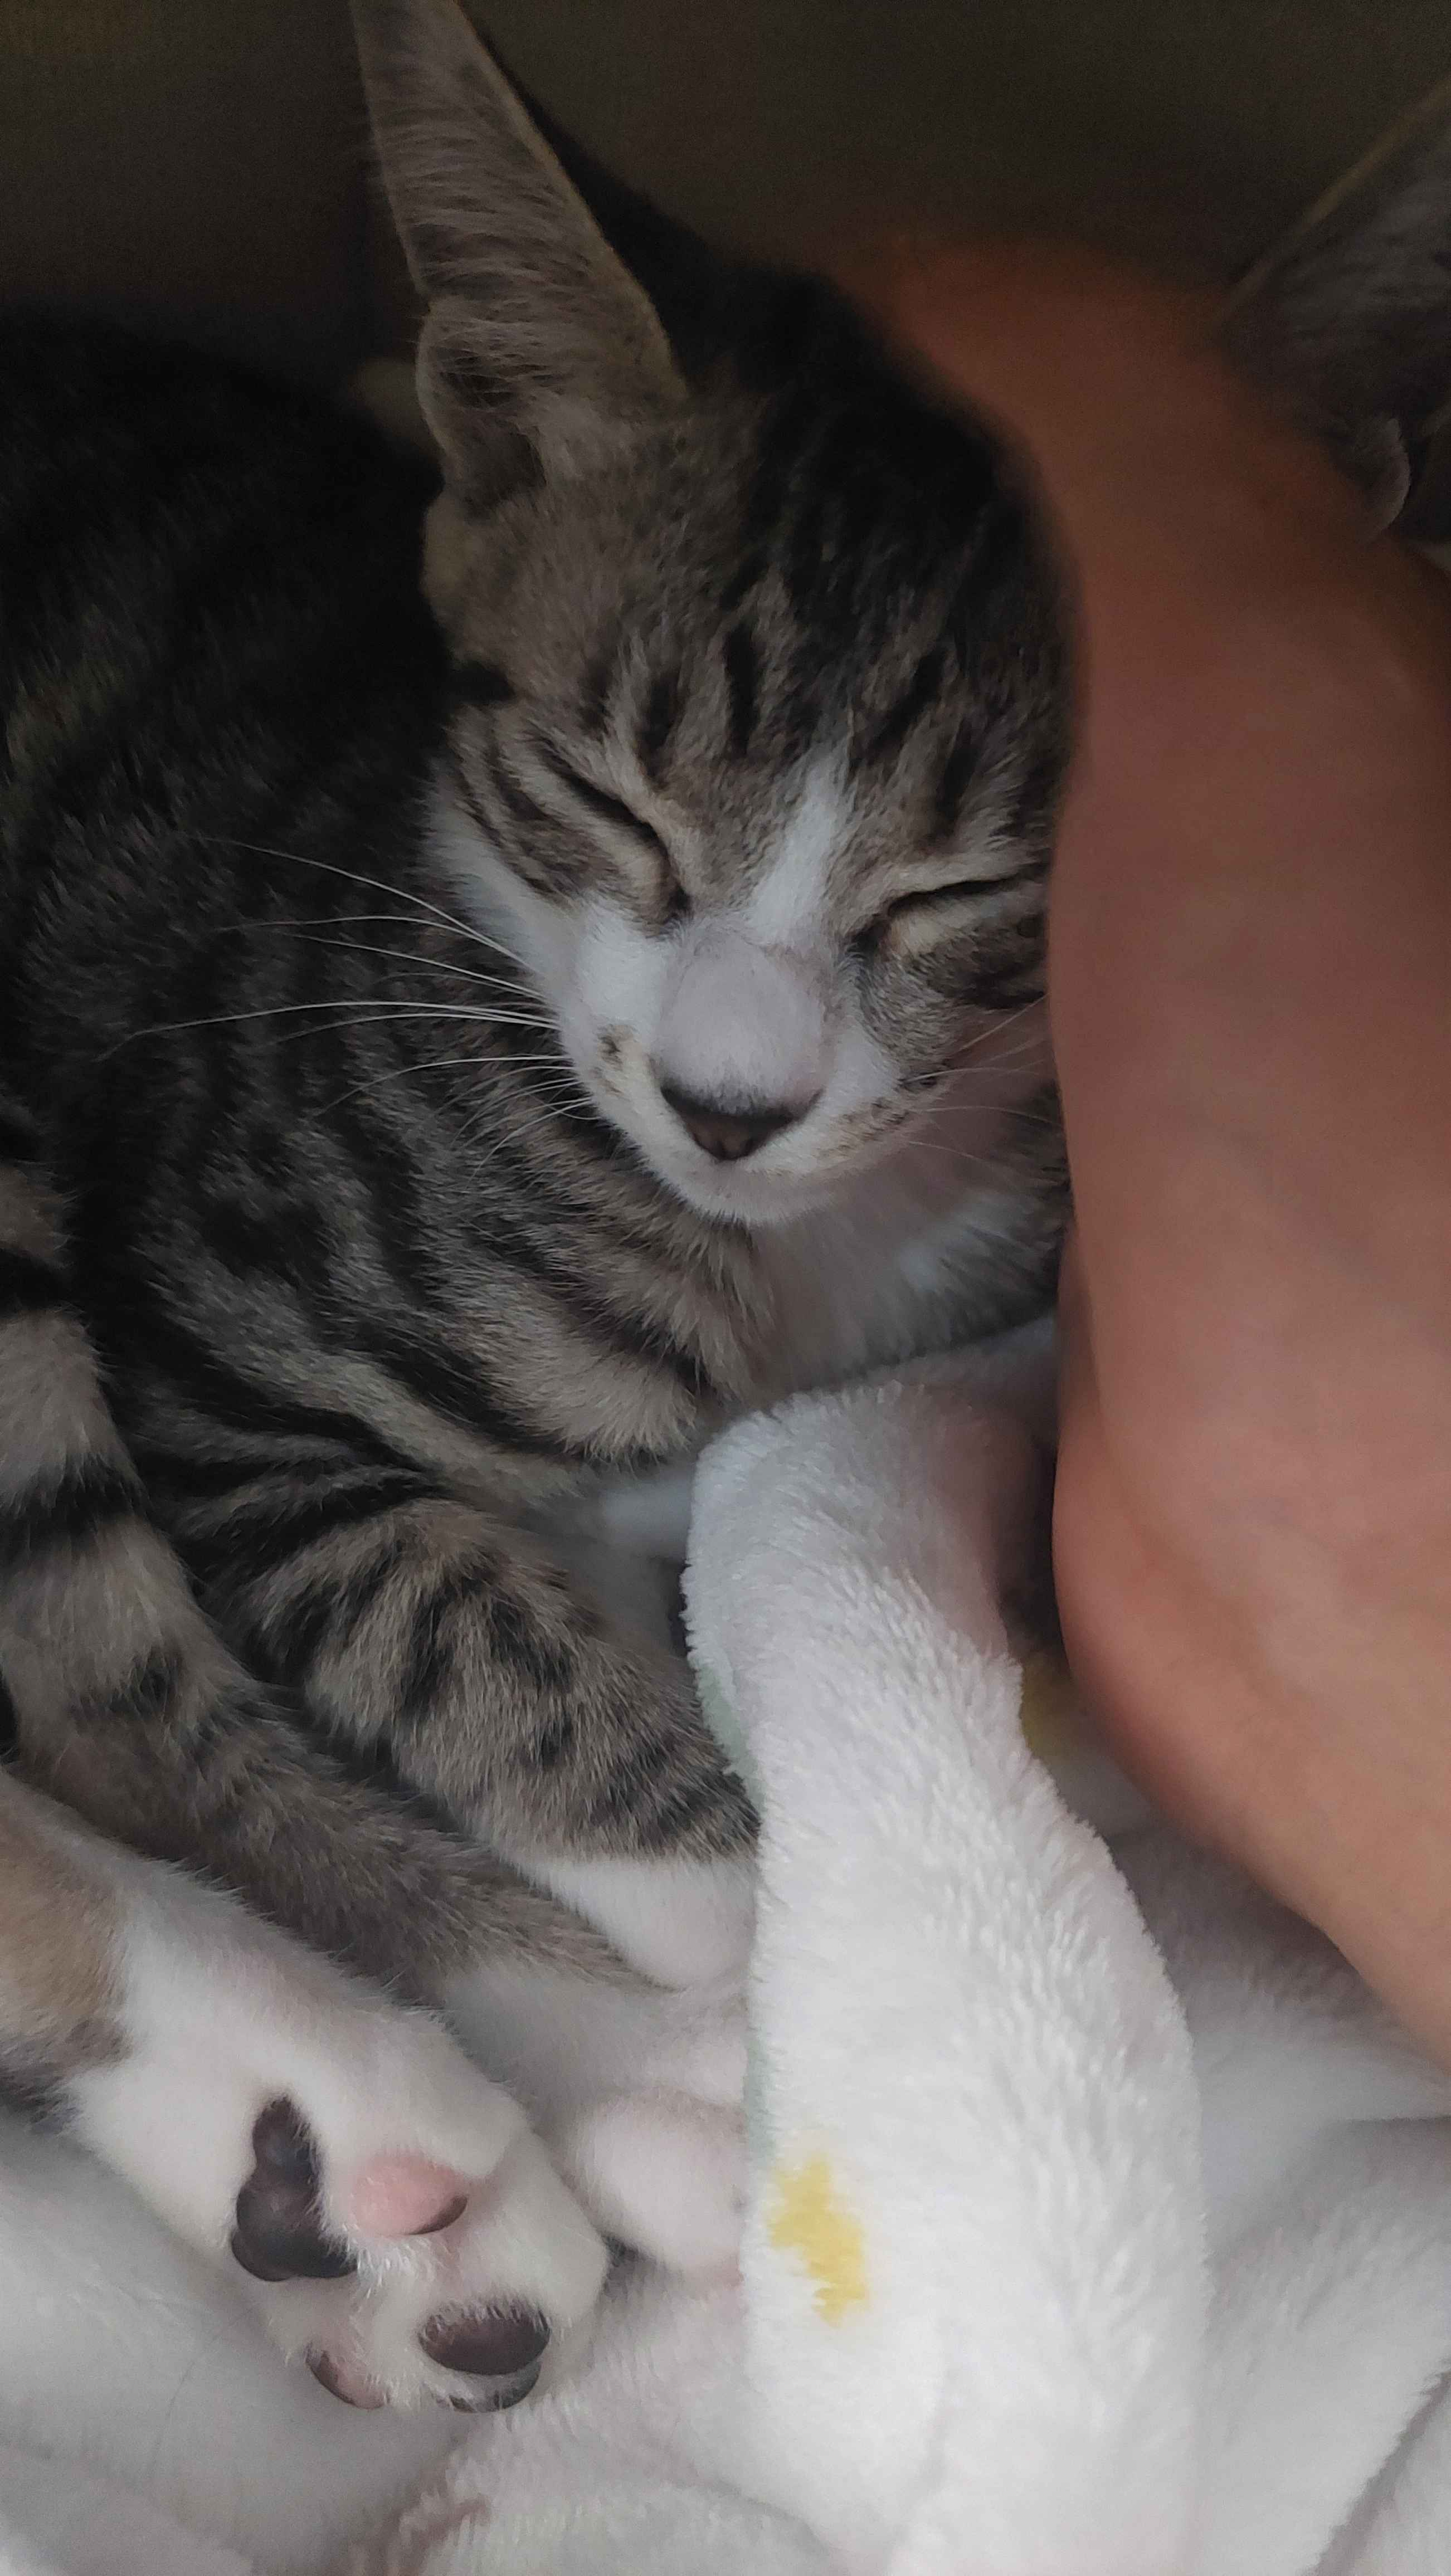
\includegraphics[width=0.65\linewidth]{photo/20250716_135406.jpg}
  \caption{이 때가 7월 16일에 찍었으니 네가 생후 3개월인 때구나. 저 때는 완전 꼬물꼬물 기어다니는 솜털뭉치였었지ㅋㅋ}
  \label{fig:2026-3-3}
\end{figure}

\newpage